% Source control vertices transcribed verbatim from the user's TikZ message.
% This file preserves the original Hobby path; separate Python source
% uses periodic cubic splines and changes P10 y by +0.07 to regularize
% its coincidence with P3. Do not interpret this reference drawing as a
% certified KPC 3D model or transfer its crossing IDs without runtime audit.
\documentclass[tikz,border=6pt]{standalone}
\usetikzlibrary{hobby,knots}
\begin{document}
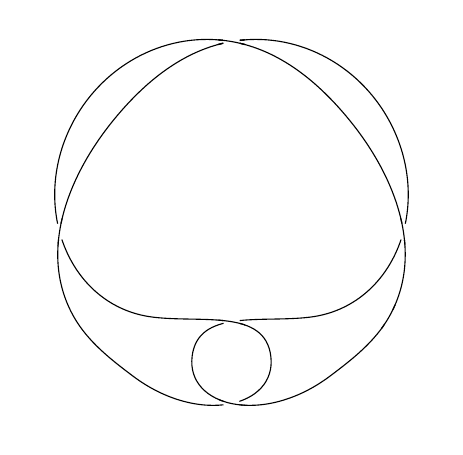
\begin{tikzpicture}[use Hobby shortcut]
\coordinate (P1) at (2, -1.50);
\coordinate (P2) at (1.50, 1);
\coordinate (P3) at (0, 2);
\coordinate (P4) at (-2, 1);
\coordinate (P5) at (-1, -1.50);
\coordinate (P6) at (0.50, -2);
\coordinate (P7) at (-1.25, -2.25);
\coordinate (P8) at (-2, -1.50);
\coordinate (P9) at (-1.50, 1);
\coordinate (P10) at (0, 2);
\coordinate (P11) at (2, 1);
\coordinate (P12) at (1, -1.50);
\coordinate (P13) at (-0.50, -2);
\coordinate (P14) at (1.25, -2.25);
\begin{knot}[consider self intersections,clip width=5pt,clip radius=3pt,ignore endpoint intersections=false,flip crossing/.list={2,4,6,8,10,12,14,16,18}]
\strand ([closed] P1)..(P2)..(P3)..(P4)..(P5)..(P6)..(P7)..(P8)..(P9)..(P10)..(P11)..(P12)..(P13)..(P14);
\end{knot}
\end{tikzpicture}
\end{document}
